\documentclass[journal]{IEEEtai}

\usepackage[colorlinks,urlcolor=blue,linkcolor=blue,citecolor=blue]{hyperref}

\usepackage{color,array}

\usepackage{graphicx}

%% \jvol{XX}
%% \jnum{XX}
%% \paper{1234567}
%% \pubyear{2020}
%% \publisheddate{xxxx 00, 0000}
%% \currentdate{xxxx 00, 0000}
%% \doiinfo{TQE.2020.Doi Number}

\newtheorem{theorem}{Theorem}
\newtheorem{lemma}{Lemma}
\setcounter{page}{1}
%% \setcounter{secnumdepth}{0}


\begin{document}


\title{Generative AI and the Riemann zeta zero distribution} 


\author{Placeholder, for double blind review
\thanks{This paragraph of the first footnote will contain the date on which you submitted your paper for review.  }
\thanks{Placeholder, for double blind review}
\thanks{This paragraph will include the Associate Editor who handled your paper.}}

\markboth{Journal of IEEE Transactions on Artificial Intelligence, Vol. 00, No. 0, Month 2020}
{First A. Author \MakeLowercase{\textit{et al.}}: Bare Demo of IEEEtai.cls for IEEE Journals of IEEE Transactions on Artificial Intelligence}

\maketitle

\begin{abstract}
The Transformer model of Generative AI introduced attention mechanisms that has had important successes in natural language processing.  We applied it for predicting the distribution of Riemann zeta zero counts on consecutive Gram intervals. The results are very good. We get accuracies of $0.998$ in predicting a sequence of ten consecutive zero counts. The input for the prediction is a sequence of the preceeding ten zero counts on sequential Gram intervals. We tested with two ranges of Riemann zeta zeros, t (height along critical axis for Riemann zeta function) = $10^{12}$ and t = $10^{28}$. The $0.998$ comes about because the intervals with $3$ or more zeros are rare. With special training for rare events, we can get essentially completely accurate prediction. One surprising result is that the model trained on a small amount of data at $10^{28}$ accurately predicts the behaviour $16$ orders of magnitude away, at $10^{12}$. The high prediction accuracy was unexpected. We present arguments that the 100\% accurate predictions cannot continue indefinitely. Our study shows that applying the technique to more complex problems has great promise. We have used very minimal computer resources compared to typical models in language applications. With access to better resources, we can attack much more important problems. 
\end{abstract}

\begin{IEEEImpStatement}
Our application of the Transformer model, renowned for its attention mechanisms in natural language processing, marks a significant breakthrough in predicting the distribution of Riemann zeta zero counts on consecutive Gram intervals. Achieving accuracies as high as $0.998$ in forecasting sequences of ten consecutive zero counts underscores the model's robustness and effectiveness in this specialized domain. By focusing on rare events — intervals with three or more zeros — and employing tailored training strategies, we achieved near-perfect predictions, showcasing the Transformer's adaptability beyond traditional linguistic tasks. Moreover, our study demonstrates promising potential for applying these techniques to more intricate problems, leveraging minimal computational resources compared to standard language models. With enhanced computational capabilities, we anticipate tackling even more impactful challenges, highlighting the transformative impact of advanced AI methodologies in mathematical research and beyond.

\end{IEEEImpStatement}

\begin{IEEEkeywords}
Attention, Generative AI, Riemann zeta, Transformer Architecture
\end{IEEEkeywords}



\section{Introduction}

\IEEEPARstart{T}{he}  Transformer model~\cite{vaswani2017attention} introduced attention mechanisms that revolutionized natural language processing (NLP).
Recent advancements \cite{radford2019language,brown2020language} include significant improvements in few-shot learning capabilities.
The effectiveness of transfer learning using a unified text-to-text Transformer approach is studied in \cite{raffel2019exploring}.
Transformer-XL, described in \cite{dai2019transformerxl}, extends the Transformer architecture to handle longer contexts in language modeling tasks.
Transformer-XH, proposed by \cite{zhang2019transformerxh}, addresses multi-hop question answering with explanation capabilities. 

The key concept underlying the advances in NLP is Attention. In Attention when the model is predicting the next word it searches for a set of positions in the source sentence where the most relevant information is concentrated. 
Consider the sentence ``Amidst the cacophony of bustling city streets, where the relentless symphony of car horns blares incessantly, echoing through the labyrinthine alleyways adorned with vibrant graffiti, there lies a quaint cafe nestled in a quiet corner, its cozy interior exuding an inviting warmth that beckons weary souls seeking solace from the frenetic pace of urban life". The ``cacophony" and ``quaint cafe" are separated in position, however, they are closely related and the relation is important to understand the sentence. The Attention concept brings out this interacton.

Earlier models in NLP used for sequence-to-sequence learning relied on Recurrent Neural Networks which are computationnally expensive. They had to process sequences step by step, whereas Transformers only need to look once at the whole sequence, moving the time complexity from O(n) to O(1). The Transformer lends itself to parallelization. 

Given the success of generative AI in extracting patterns in NLP, there is potential to apply similar techniques to challenging problems such as the Riemann zeta function.
Machine learning has been used in mathematical applications. An early example is  Ref.~\cite{osneural}. This was followed by \cite{he2022sato,HeMLNF,HeStringLandscape,
Vartziotis2023,Kim2022}. In what follows we apply Generative AI to the Riemann zeta zeros.
We found three surprising results.

\begin{enumerate}
    \item With a model trained on just $5000$ zeros, we get $100\%$ accuracy on two sets of samples consisting of $200000$ zeros each.
    
    \item The two sets of samples are separated by $16$ orders of magnitude.
    
    \item While the first two items might seem to indicate that the pattern of zero counts is regular, we show in the Appendix that in fact the zero counts are not bounded and take on arbitrarily large values, and also long sequences of intervals with no zeros also occur for large enough heights on the critical axis. 
    
\end{enumerate}

\section{Background}

For those who do not wish to get too deep into Riemann zeta theory, just ignore all the discussion about the theory, and understand that we have a sequence of counts, and we wish to see how well Generative AI does in predicting the pattern underlying the sequence of counts. To make this more concrete, in Table~\ref{tab:sequence} we show a sequence of zero counts on consecutive Gram intervals. The sequence of counts has been broken up into separate rows, merely for convenience in presentation. The problem we solve is: given a sequence of ten such intervals, predict the zero counts on the next set of ten successive intervals.
For more detail on Gram intervals, see \cite{Shanker 2018a}.

\subsection{Riemann zeta function}


\begin{table}
\centering \(\begin{array}{ccccccccccccccc}
\hline
2& 0& 1& 2& 0& 1& 1& 1& 0& 2& 1& 0& 1& 2& 1 \\
2& 0& 1& 1& 1& 2& 0& 1& 1& 1& 0& 2& 1& 1& 1 \\
0& 2& 1& 2& 1& 0& 1& 1& 1& 1& 1& 1& 1& 1& 1 \\
1& 1& 1& 1& 1& 1& 1& 0& 1& 2& 1& 1& 1& 1& 0 \\
2& 1& 1& 0& 3& 1& 0& 2& 1& 1& 0& 1& 1& 1& 1 \\
\hline
\end{array}\)
\caption{Count of zeros on consecutive Gram intervals (shown on multiple lines for convenience).} 
\label{tab:sequence}
\end{table}


The Riemann Zeta function is defined for $\mathrm{Re} (s) > 1$ by
\begin{equation}
\zeta ( s ) \, = \, \sum^{\infty}_{n = 1} \; n^{-s} \, = \, \prod_{p \in primes} \;
\left( 1 - p^{-s} \right)^{-1}.
\label{eqRie}
\end{equation}

Eq.~(\ref{eqRie})  converges for $\mathrm{Re} (s) > 1$.  
 $\zeta ( s )$ has a  continuation
to the complex plane. The zeroes of the Riemann zeta function can be written as $1/2 + i t$. The Riemann Hypothesis  
is that $t$ is real for the non-trivial zeroes. The line of zeros is called the critical axis.

\subsection{Gram points}
The critical axis can be divided into Gram intervals. 
We define
\begin{equation}
\theta(t) = arg (\pi^{-it/2} \Gamma(\frac{1}{4} + \frac{it}{2})), 
\label{eq:theta}
\end{equation}
where the argument is defined by continuous variation of $t$ starting with the value $0$ at $t = 0$.
For large $t$ $\theta$ has the asymptotic expansion
\begin{equation}
\theta(t) = \frac{t}{2}\ln (\frac{t}{2\pi}) - \frac{t}{2} - \frac{\pi}{8} + \frac{1}{48t} - \frac{1}{5760t^3}. 
\label{eq:thetaAsymptotic}
\end{equation}
 When $t \ge 7$, the $\theta$ function Eq.(\ref{eq:theta}) is monotonic increasing. 
For $n \ge 1$, the $n-th$ Gram point $g_n$ is defined as the unique solution $> 7$ to
$\theta (g_n) = n\pi$.
The Gram points are as dense as the zeros of $\zeta(s)$ but are much more regularly distributed. They divide the critical axis into Gram intervals. On average, each Gram interval contains one zero of the Riemann zeta function.

\subsection{\label{seccounts}Zero counts on Gram intervals}
 Odlyzko~\cite{Odlyzko 1992} made a conjecture regarding the distribution of Gram intervals that contain a given number of zeros. 
Table~\ref{tab:intervalzeros} shows the counts of Gram intervals that contain $m$ zeros, for samples at heights  $t=10^{12}$ and $t=10^{28}$, and the  expected values for the counts from Odlyzko's prediction. We use the zeros from Ref~\cite{hiary 2010}. The last row is from Table 2.13.3 of Ref.~\cite{Odlyzko 1992}. The agreement with Odlyzko's prediction is very good. 
Asymptotically, for the Riemann zeta function the mean number of 
zeros with height less than $t$ 
is~\cite{Edwards(1974)}
\begin{equation}  
N (t) = (t/2\pi)(ln(t/2\pi)-1)-\frac{7}{8}.
\label{eq:Rnumber}
\end{equation}
Thus, the mean spacing of the zeros at height $t$ is 
$2\pi(\ln (t/2\pi))^{-1}$. For the range of $t$ values
studied by us this spacing is essentially constant.
The error in the approximation $N (t) - \pi^{-1}\theta(t) -1$ is denoted in the literature by $S(t)$. On average, $S(t)$ approaches zero. However, it takes on arbitrarily large positive and negative values for large $t$, i.e., it is not bounded above or below.

\begin{table}
\centering \(\begin{array}{lllll}\\
\hline
 &count = 0&count = 1&count = 2&count = 3\\
\hline
t = 10^{12}&0.14880&0.70440&0.14482&0.00199\\
t = 10^{28}&0.16192&0.67815&0.15795&0.00199\\
Odlyzko&0.17022&0.66143&0.16640&0.00186\\
\hline
\end{array}\)
\caption{Distribution of Gram intervals that contain $m$ zeros at  $t=10^{12}$.} 
\label{tab:intervalzeros}
\end{table}


\section{Generating the dataset}

theta and counts


\section{Methodology}


\subsection{\label{sec3.1} Choosing the Model}
Typical applications of Transformers involve use of huge amounts of computing resources and data to learn, for example, Natural Language processing. Here, we extend the application to a mathematical domain, the Riemann Zeta function. Since this is a new domain of application, we build a very simple model to study how well the simple model performs. For the Transformer model we build upon the presentation in  Ref~\cite{BenjaminEtienne}. The code for our implementation is available at 
 Ref~\cite{shankergit}.
We use PyTorch (\url{https://pytorch.org/})  due to its flexibility and ease of use.


history. start with $10^{12}$. First zero   at $10^{12} + 244.158907$. reached 0.998, plateaued. 


\begin{table}
\centering \(\begin{array}{ccc}
\hline
\hline
Training  & Training &Validation  \\
set     &accuracy&accuracy\\
\hline
1  & 0.675 & 0.716 \\

2  & 0.914 & 0.998 \\
\hline
\end{array}\)
\caption{Training and validation accuracies $t=10^{12}$}
\label{tab:accuracies12}
\end{table}

\subsection{\label{10E12} $t=10^{12}$}

We began the study with the zeros at $t=10^{12}$.
We did two rounds of training and validation. In the first round we use $6400$ samples for training, and $10000$ samples for validation.   The average training and validation accuracies are $0.675$ and $0.716$ respectively (Table~\ref{tab:accuracies12}).

In the second round we use $8400$ samples for training, and $10000$ samples for validation. The average training and validation accuracies are $0.914$ and $0.998$ respectively. Since the second round of training uses the model trained on the first round, the accuracy is higher. We tried different combinations of parameters, but the overall accuracy plateaued at $0.998$.


\begin{figure}
\centerline{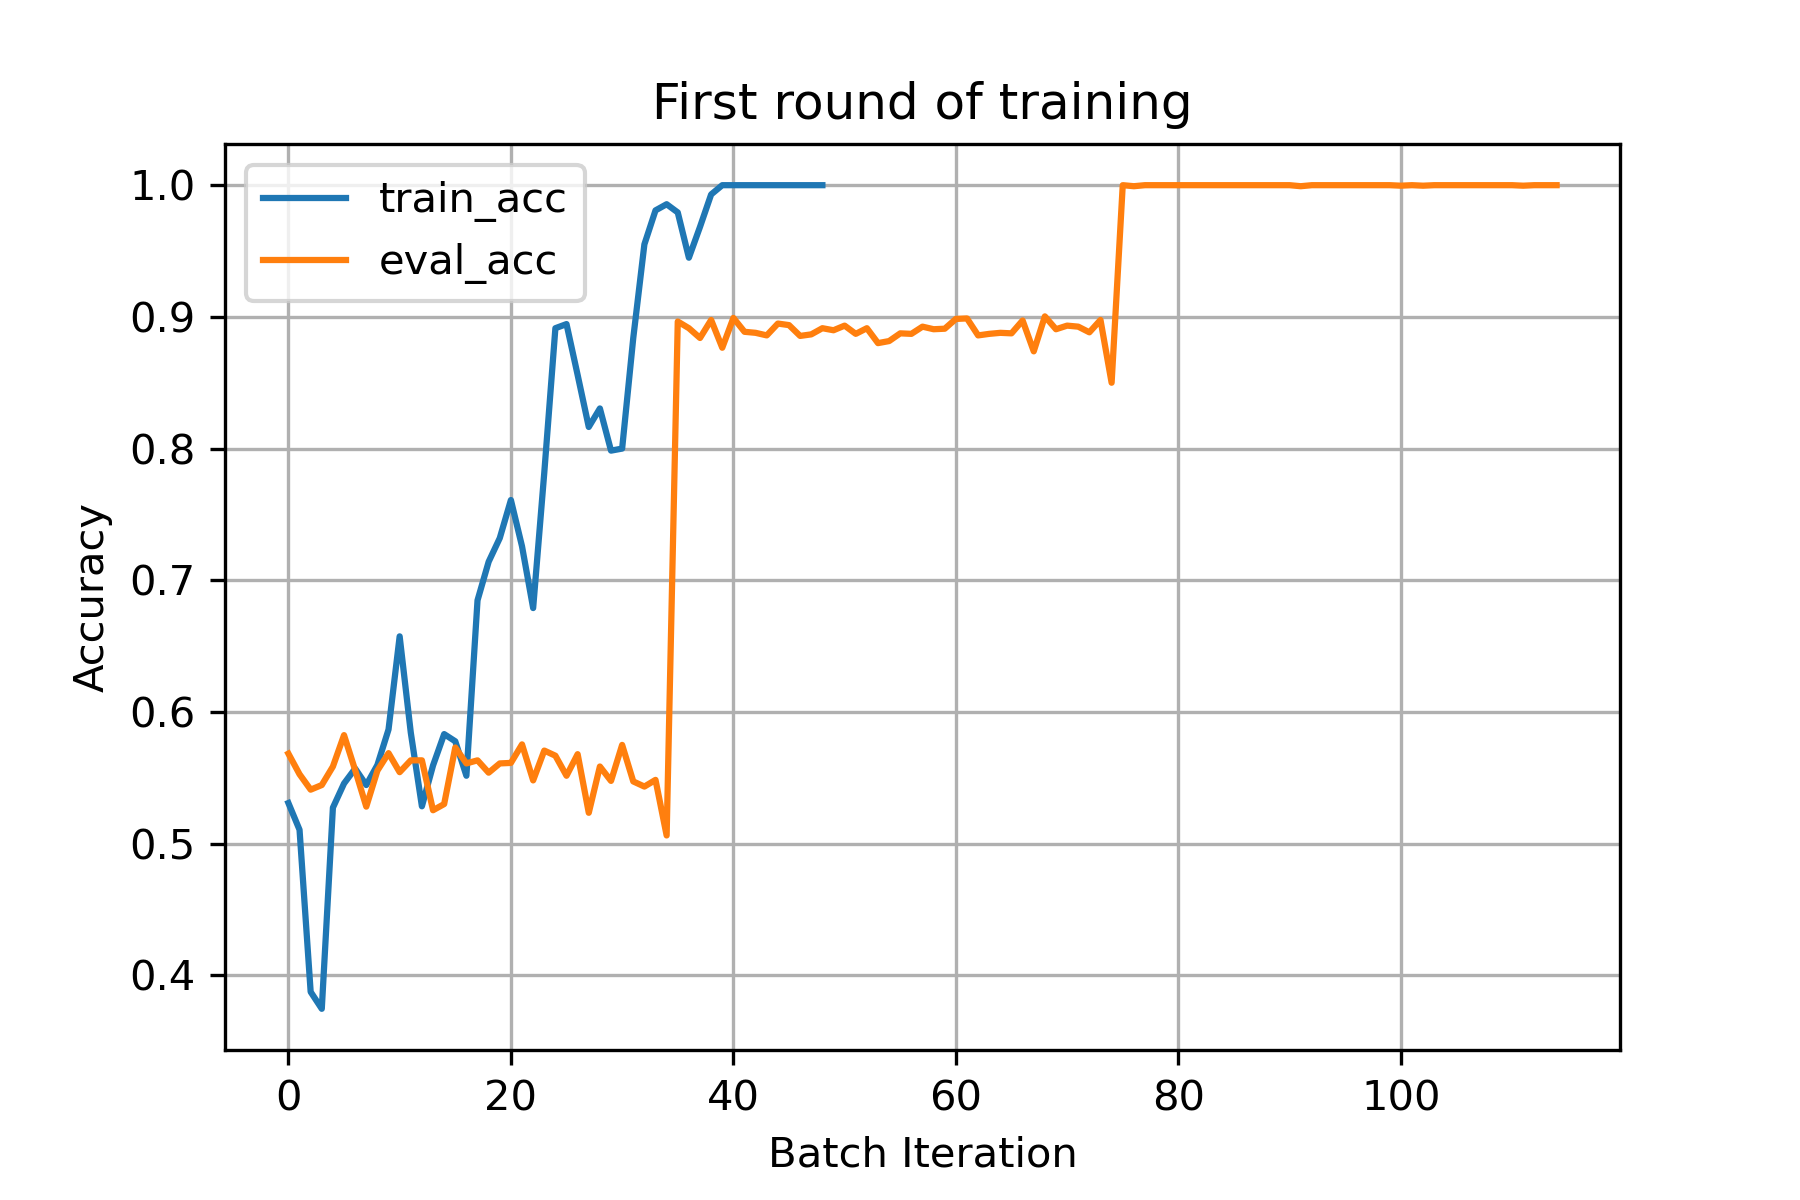
\includegraphics[width=18.5pc]{Figure1.png}}
\caption{Training and validation accuracies for the rare events sample. The data is for 
the three epochs of the first round of training.}
\label{fig:1}
\end{figure}


\section{Analysis}



\begin{table}
\centering \(\begin{array}{ccc}
\hline
\hline
Training  & Training &Validation  \\
set     &accuracy&accuracy\\
\hline
1, epoch 1  & 0.519 & 0.588 \\

1, epoch 2  & 0.797 & 0.900 \\
1, epoch 3  & 0.983 & 1.000 \\

2  & 1.000 & 1.000 \\
\hline
\end{array}\)
\caption{Training and validation accuracies for dataset containing rare data. Round 1 
sample size is 4500, and round 2 sample size is 500.}
\label{tab:accuraciesrare}
\end{table}

\begin{table}
\centering \(\begin{array}{ccc}
\hline
\hline
t     &sample~size&accuracy\\
\hline
10^{12}  & 200000 & 1.000 \\

10^{28}  & 200000 & 1.000 \\
\hline
\end{array}\)
\caption{Validation accuracies using model trained on just  rare samples}
\label{tab:validation}
\end{table}

Use 
Table of training iter and validation, ranges

\subsection{\label{rarefix}Fixing the model for rare events}
We studied in detail the $0.002$ samples where the model and the actual values deviated. 
We realized that the accuracy plateau of $0.998$ is due to the presence of rare events where the Gram interval contains $3$ or more zeros. went to $10^{28}$. only 3s enough. covers large orders of magnitude. To handle this situation, we cull samples containing such rare events from a set of $10$ million zeros at $t=10^{28}$. From the $10$ million zeros we were able to get a sample of $19616$ rare events. When we pre-train the model with this set, and then train the model on the given dataset, we get essentially completely accurate predictions (Table~\ref{tab:accuraciesrare}). Fig.~\ref{fig:1}.  Don't need round 2. Why it doesn't overtrain. (Table~\ref{tab:validation}).

cannot continue for ever.


\section{Conclusion and Future Work}

what next.


\section*{\label{appendix}Appendix}

In this appendix we show that the $100\%$ accuracy is misleading, and the zero counts are not as predictable as might originally seem. In Section~\ref{seccounts} we mentioned that
the error $S(t)$ in the approximation $N (t) - \pi^{-1}\theta(t) -1$ is not bounded above or below. $S(t)$ can be expressed in terms of the zero counts on the Gram intervals. The fact that $S(t)$ is not bounded above or below immediately implies that the zero counts on a Gram interval are also not bounded. The possible classes for the transformer model inputs and outputs are unbounded. Since the model has a finite capacity, at some point the model will not be able to predict exactly. 




\begin{thebibliography}{34}

\bibitem{vaswani2017attention}
A. Vaswani, N. Shazeer, N. Parmar, J. Uszkoreit, L. Jones, A. N. Gomez, Ł. Kaiser, and I. Polosukhin, ``Attention is all you need",  \emph{Advances in Neural Information Processing Systems (NeurIPS)}, vol. 30, pp. 5998--6008, 2017.

\bibitem{radford2019language}
A. Radford, J. Wu, R. Child, D. Luan, D. Amodei, and I. Sutskever, ``Language models are unsupervised multitask learners", \emph{OpenAI Blog}, vol. 1, no. 8, p. 9, 2019.

\bibitem{brown2020language}
T. B. Brown, B. Mann, N. Ryder, M. Subbiah, J. Kaplan, P. Dhariwal, A. Neelakantan, P. Shyam, G. Sastry, A. Askell, et al., ``Language models are few-shot learners",  \emph{Advances in Neural Information Processing Systems (NeurIPS)}, vol. 33, 2020.

\bibitem{raffel2019exploring}
C. Raffel, N. Shazeer, A. Roberts, K. Lee, S. Narang, M. Matena, Y. Zhou, W. Li, and P. J. Liu, ``Exploring the limits of transfer learning with a unified text-to-text transformer", \emph{arXiv preprint arXiv:1910.10683}, 2019.

\bibitem{dai2019transformerxl}
Z. Dai, Z. Yang, Y. Yang, J. Carbonell, Q. V. Le, and R. Salakhutdinov, ``Transformer-XL: Attentive language models beyond a fixed-length context",  \emph{Proceedings of the 57th Annual Meeting of the Association for Computational Linguistics (ACL)}, pp. 2978--2988, 2019.

\bibitem{zhang2019transformerxh}
Y. Zhang, Z. Gan, R. Henao, D. Shen, and L. Carin, ``Transformer-XH: Multi-hop question answering with explanation",  \emph{Advances in Neural Information Processing Systems (NeurIPS)}, vol. 32, 2019.

\bibitem{osneural} O. Shanker, ``Neural Network prediction of Riemann zeta zeros'',
\emph{Advanced Modeling and Optimization}, vol. 14, 717-728, 2012. \url{https://www.researchgate.net/publication/273945970_Neural_Network_prediction_of_Riemann_zeta_zeros}.

\bibitem{he2022sato} Y. H. He, K. H. Lee, and T. Oliver, ``Machine-learning the Sato–Tate conjecture'', \emph{Journal of Symbolic Computation}, vol. 111, 61-72, 2022.

\bibitem{HeMLNF}
Y. H. He, K. H. Lee, and T. Oliver, 
``Machine-learning number fields.",
\emph{arXiv preprint arXiv:2011.08958}, 2020.

\bibitem{HeStringLandscape}
Y. H. He,
``From the string landscape to the mathematical landscape: a machine-learning outlook."
\emph{International Workshop on Lie Theory and Its Applications in Physics}, Singapore, Springer Nature Singapore, 21-31, 2021.

\bibitem{Vartziotis2023}
D. Vartziotis, G. Dasoulas,  and  F. Pausinger,
``Learn2Extend: Extending sequences by retaining their statistical properties with mixture models.",
\emph{arXiv preprint arXiv:2312.01507}, 2023.

\bibitem{Kim2022}
E. Kim, 
``Deep learning-based approximation of Goldbach partition function.",
\emph{Discrete Mathematics, Algorithms and Applications} vol. 14,  2150152, 2022.

\bibitem{Shanker 2018a} O. Shanker, 
``Good-to-Bad Gram Point Ratio For Riemann Zeta Function",
\emph{Experimental Mathematics}, vol. 30, 76-85, 
\url{https://doi.org/10.1080/10586458.2018.1492474}, 2021

\bibitem{Odlyzko 1992}  A. Odlyzko,
``The $10^{20}$-th Zero of the Riemann Zeta
Function and 175 Million of its Neighbors", report,
\url{http://www.dtc.umn.edu/~odlyzko/unpublished/zeta.10to20.1992.pdf}, 1992

\bibitem{hiary 2010} G. A. Hiary,
``An amortized-complexity method to compute the Riemann zeta function", 
{\it Mathematics of Computation} {\bf80}, 1785-1796, 2011

\bibitem {Edwards(1974)} H. M. Edwards, ``Riemann's Zeta Function,'' 
Academic Press,  1974.

\bibitem{BenjaminEtienne} Benjamin Etienne, 
``A Complete Guide to Write your own Transformers'',
 \emph{Towards Data Science},
\url{https://towardsdatascience.com/a-complete-guide-to-write-your-own-transformers-29e23f371ddd}, 
2024. 

\bibitem{shankergit} placeholder, 
Source code on github,
2024. 


\end{thebibliography}






\begin{IEEEbiography}{First A. Author}{\space}   placeholder, for double blind review
\end{IEEEbiography}


\end{document}
